\section{Antenna Design 2 -- Triangle-Feed Antenna}

\begin{figure}[htbp]
    \begin{subfigure}[b]{0.49\linewidth}
        \centering
        \includegraphics{img/tech_sol/trianglefeed/technical}
        \caption{Technical drawing.}
        \label{fig:ant2technical}
    \end{subfigure}
    \hfill
    \begin{subfigure}[b]{0.49\linewidth}
        \centering
        \includegraphics{img/tech_sol/schematic_tuning_1}\\[1cm]
        \footnotesize
        \begin{tabular}{|l|l|l|l|}
            \hline
            & $C_1$ & $L_1$ & $C_2$ \\
            \hline
            Top antenna & \SI{3.45}{pF} & \SI{7.89}{nH} & $[0.3,2.9]\,$pF\\
            Side antenna & \SI{2.42}{pF} & \SI{5.69}{nH} & $[0.3,2.9]\,$pF\\
            \hline
        \end{tabular}
        \caption{Tuning/matching circuit.}
        \label{fig:ant2schematic}
    \end{subfigure}
    \caption{Technical drawing and tuning circuit for the antenna.  The antennas are built on FR-4 board using \SI{35}{\micro\meter} copper. There is a matching circuit as shown for each of the two feeds.}
    \label{fig:ant2techschem}
\end{figure}

\begin{figure}[htbp]
    \begin{subfigure}{0.49\linewidth}
        \centering
        \includegraphics{img/tech_sol/trianglefeed/Csh1s11.pdf}
        \caption{$S_{11}$ with $C_2=\SI{0.3}{pF}$ and $C_1$ varying from \SI{0.3}{pF} to \SI{2.9}{pF}.}
    \end{subfigure}
    \hfill
    \begin{subfigure}{0.49\linewidth}
        \centering
        \includegraphics{img/tech_sol/trianglefeed/Csh2s22.pdf}
        \caption{$S_{22}$ with $C_1=\SI{0.3}{pF}$ and $C_2$ varying from \SI{0.3}{pF} to \SI{2.9}{pF}.}
    \end{subfigure}
    \\
    \begin{subfigure}{0.49\linewidth}
        \centering
        \includegraphics{img/tech_sol/trianglefeed/Csh1s21.pdf}
        \caption{$S_{21}$ with $C_2=\SI{0.3}{pF}$ and $C_1$ varying from \SI{0.3}{pF} to \SI{2.9}{pF}.}
    \end{subfigure}
    \hfill
    \begin{subfigure}{0.49\linewidth}
        \centering
        \includegraphics{img/tech_sol/trianglefeed/Csh2s21.pdf}
        \caption{$S_{21}$ with $C_1=\SI{0.3}{pF}$ and $C_2$ varying from \SI{0.3}{pF} to \SI{2.9}{pF}.}
    \end{subfigure}
    \caption{Parameter sweeps for tuning the shunt capacitor of each antenna, $C_{1}$ and $C_{2}$ for port 1 and 2, respectively. Port 1 is the top antenna and port 2 is the side antenna. The capacitor values are changed in \SI{0.2}{pF} steps.}
    \label{fig:ant2sweeps}
\end{figure}
